%!TEX root = ../Main.tex

\chapter{Results}
An important aspect of HW/SW co-design is to identify potential bottlenecks of software tasks and to determine if that task is suitable for hardware acceleration. For this project it was determined that the calculation of distance between the points to be the most demanding task. On \cref{fig:timing_pie} a piechart shows the three most demanding tasks as the amount of clock cycles each process uses for one iteration of the genetic algorithm. 

\begin{figure}[H]
	\centering
	{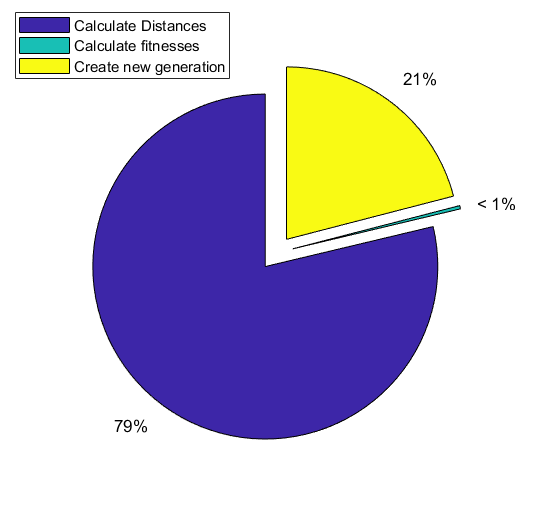
\includegraphics[width=\textwidth]{Images/timing_pieChart.png}}\\[0.5cm]
	\caption{Most demanding tasks in \%}
	\label{fig:timing_pie}
\end{figure}





\begin{figure}[H]
	\centering
	{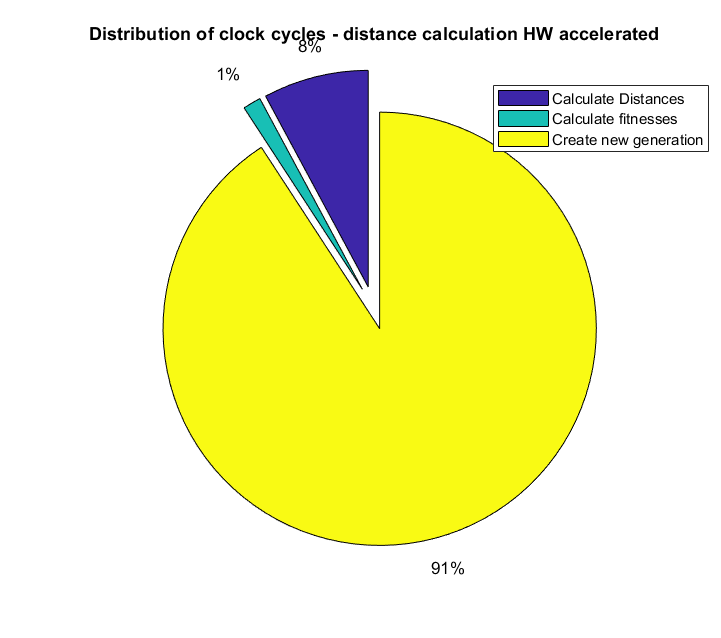
\includegraphics[width=\textwidth]{Images/cycle_distribution_HW_accelerated.png}}\\[0.5cm]
	\caption{Most demanding tasks in \% after hardware acceleration}
	\label{fig:timing_pie_hw}
\end{figure}
